\chapter{Modelo propuesto por Watson y Crick}
\label{modelo}

James Watson y Francis Crick dedujeron un modelo estructural tridimensional para el DNA a partir de datos existentes a cerca del mismo. 
Los datos conocidos era:
\begin{enumerate}
	\item Se sabía que la molécula de DNA era muy grande, también muy larga y delgada, y que estaba compuesta de nucleótidos que contenían las bases 				nitrogenadas: adenina, guanina, timina y citosina.
	\item De acuedo con la hipótesis de Levene, se suponía que estos nucleótidos estaban ensamblados en unidades repetidas de cuatro.
	\item El químico L. Pauling había propuesto en 1950, que las cadenas de aminoácidos que componen las proteínas están dispuestas a menudo en forma
			de hélice y que se mantiene así por puentes de hidrógeno. Pauling había sugerido que la estructura del DNA podía ser similar.
	\item Los físicos Maurice Wilkins y Rosalind Franklin habían aplicado la técnica de difracción de rayos X al estudio del DNA. Las fotografías 				obtenidas mostraban patrones que casi con certeza reflejaban los giros de una hélice gigante.
	\item  Datos que indicaban que, dentro del error experimental, la cantidad de adenina (A) es igual que la de timina (T) y que la de guanina (G) es 				igual que la de citosina (C): A=T y G=C. (Chargaff)
\end{enumerate}
A partir de estos datos, algunos de ellos contradictorios, Watson y Crick intentaron construir un modelo de DNA que concordara con los hechos conocidos y explicara su papel biológico. Los dos científicos fueron capaces de deducir que el DNA es una doble hélice, entrelazada y sumamente larga.
Algunas de las conclusiones fueron:
\begin{itemize}
	\item Las cadenas tienen dirección y corren en direcciones opuestas, es decir, la dirección desde el extremo 5' al 3' de cada cadena es opuesta y se 				dice que las cadenas son \textit{antiparalelas}.
	\item Los nucleótidos situados en cualquiera de las cadenas de la doble hélice podían acoplarse en cualquier orden o secuencia, aunque su secuencia 			determina el orden de los nucleótidos de la otra cadena. Esto es necesario, porque las cadenas son complementarias. Por ejemplo: la cadena 				complementaria de la secuencia \textbf{(5')- T T C A G T A C A T T G C C A-(3')} tiene que tener la cadena de nucleótidos \textbf{(3')- A A G 				T C A T G T A A C G G T-(5')}.
	\item No solamente las purinas no podrían aparearse con purinas, ni las pirimidinas con pirimidinas, sino que, a causa de las estructuras particulares 				de las bases, la adenina sólo podía aparearse con la timina, formando dos puentes de hidrógeno (A=T) y la guanina solamente con la citosina, 				formando tres puentes de hidrógeno (G=C). Las bases apareadas eran complementarias.
\end{itemize}

\begin{figure} [h]
	\begin{center}
		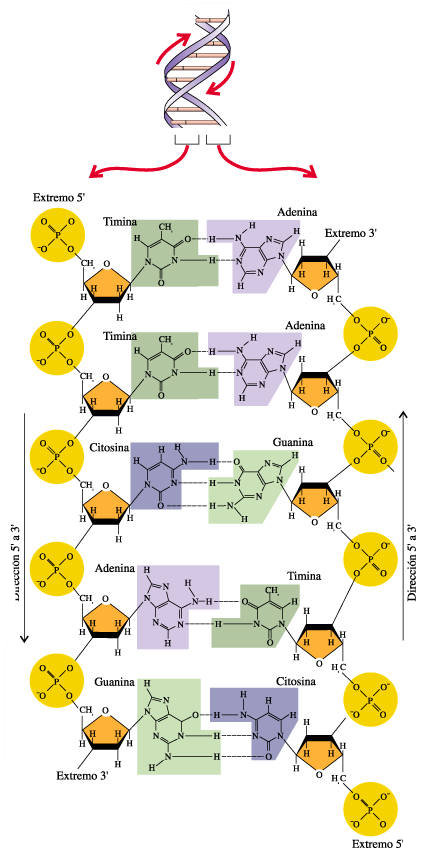
\includegraphics[width=2.2209in,height=3.2000in]{image/watson.jpg}
		\caption{Modelo estructural Watson-Crick [19].}
	\end{center}
\end{figure}	

